% =====================================================================
% Template LaTeX – Traces distribuées aux étudiants
% Auteur : (à compléter)
% Compilation : pdflatex/xelatex (pdflatex recommandé ici)
% =====================================================================
\documentclass[11pt,a4paper]{report}

% -------------------- Encodage & langue --------------------
\usepackage[T1]{fontenc}
\usepackage[utf8]{inputenc}
\usepackage[french]{babel}
\usepackage{lmodern}
\usepackage{microtype}
\usepackage{amsmath, amssymb}
\usepackage{multicol}
\usepackage{enumitem}

\usepackage{amsfonts}
\usepackage[version=4]{mhchem}
\usepackage{stmaryrd}
\usepackage{graphicx}
\usepackage[export]{adjustbox}
\graphicspath{ {./images/} }
\usepackage{caption}
\usepackage{multirow}

% -------------------- Mise en page --------------------------
\usepackage[a4paper,margin=2cm]{geometry}
\usepackage{fancyhdr}
\usepackage{parskip}      % espace entre paragraphes
\setlength{\parindent}{0pt}

% -------------------- Couleurs & liens ----------------------
\usepackage{xcolor}
\definecolor{Theme}{HTML}{0E7490} % teal-700
\definecolor{ThemeLight}{HTML}{E0F2F1}
\definecolor{Accent}{HTML}{F59E0B} % amber-500
\definecolor{Gray}{HTML}{374151}
\usepackage[colorlinks=true,linkcolor=Theme,urlcolor=Theme,citecolor=Theme]{hyperref}

% -------------------- Graphiques / décor --------------------
\usepackage{tikz}
\usetikzlibrary{patterns,positioning,calc}
\usepackage{graphicx}
\usepackage{tcolorbox}
\tcbuselibrary{skins,breakable,hooks,most}
\usepackage{fontawesome5}

% -------------------- Titres -------------------------------
\usepackage{titlesec}
\titleformat{\chapter}[display]
  {\Huge\bfseries\color{Theme}}
  {\filright\rule{0.75\linewidth}{1.2pt}\\[3pt]{Algèbre linéaire - Chapitre~\thechapter}}
  {0.2ex}
  {\filright}
  [\vspace{0.1ex}\rule{0.35\linewidth}{1.2pt}]

\titleformat{\section}
  {\Large\bfseries\color{Gray}}
  {\thesection}{0.6em}{}

% -------------------- En-têtes / pieds ---------------------
\pagestyle{fancy}
\fancyhf{}
\fancyhead[L]{\color{Gray}\leftmark}
\fancyhead[R]{\color{Gray}\textit{MEF - 2025/2026}}
\fancyfoot[R]{\color{Gray}\small p.\ \thepage}
\renewcommand{\headrulewidth}{0pt}
\renewcommand{\footrulewidth}{0pt}

% -------------------- Macros utilitaires -------------------


% Tcolorboxes stylisées
\tcbset{tracebox/.style={breakable,enhanced,sharp corners,boxrule=0pt,frame hidden,arc=2mm,
  colback=white,coltitle=black,fonttitle=\bfseries\large,
  borderline west={2mm}{0pt}{Theme},
  before skip=8pt,after skip=8pt,drop fuzzy shadow}}

\newtcolorbox{resumeBox}{tracebox,title={\faStickyNote\quad Résumé des idées}}
\newtcolorbox{rappelsBox}{tracebox,title={\faRedo\quad Ce que je dois savoir }}
\newtcolorbox{exempleBox}{tracebox,title={\faChalkboardTeacher\quad Exemple vu ensemble}}

% Encadré « Formules & illustrations »
\newtcolorbox{formulesBox}{tracebox,title={\faCalculator\quad Formules \& illustrations},colback=ThemeLight}

% Astuce : puces clean
\newenvironment{niceitemize}{\begin{itemize}\setlength{\itemsep}{0.25em}\color{Gray}}{\end{itemize}}

% Raccourci pour une « Trace » complète
% Usage : \TraceSection{Titre}{Objectif court}
\newcommand{\TraceSection}[2]{%
  
}

% -------------------- Page de titre ------------------------
\title{\textbf{Traces de cours}\\\large (résumés, formules, exemples, mini-exercices)}
\author{ TECE - 2025/2026 }
\date{\today}


\makeatletter
\renewcommand{\thesubsection}{\arabic{subsection}}
\renewcommand{\p@subsection}{}% supprime le préfixe section/chapter dans \ref
% Si vous voulez la même chose pour les sous-sous-sections :
% \renewcommand{\thesubsubsection}{\arabic{subsubsection}}
% \renewcommand{\p@subsubsection}{}
\makeatother

\usepackage{mdframed}
\usepackage{ifthen}

% \usepackage[sf]{titlesec}
% Définition de la variable pour afficher les corrections
\newboolean{showSolutions}
% Décommentez la ligne suivante pour afficher les solutions
\input \jobname.adr
% -------------------- Document ----------------------------
\begin{document}

\captionsetup{singlelinecheck=false}
\section*{Problème}
On considère une barre de longueur $2 L$, constituée de deux barres de longueur égale :

\begin{itemize}
  \item Barre $AB$ (acier) : $L=6 \mathrm{~m} ; E_{1}=210000 \mathrm{MPa}, A_{1}=0.001 \mathrm{~m}^{2}$
  \item Barre $BC$ (aluminium) : $L=6 \mathrm{~m} ; E_{2}=70000 \mathrm{MPa}, A_{2}=0.003 \mathrm{~m}^{2}$
\end{itemize}

La barre $1$ est soumise à un chargement constant $p=100 \mathrm{kN} / \mathrm{m}$.

\begin{center}
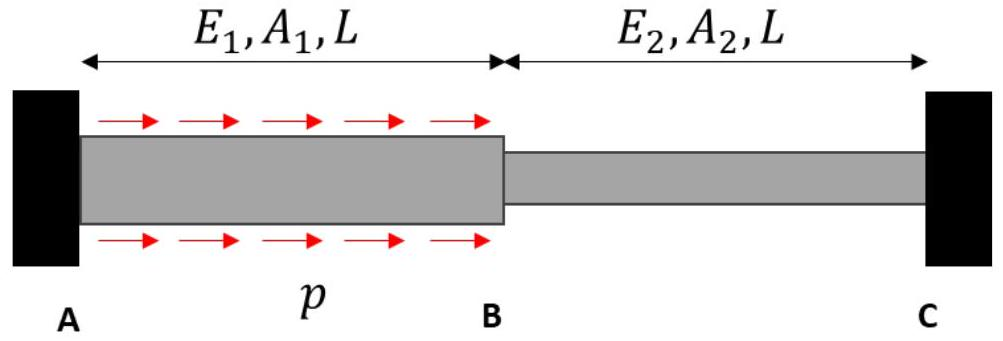
\includegraphics[max width=0.9\textwidth, center]{2025_10_03_26e11264345fd9bad5cag-1(2)}
\end{center}

On cherche à déterminer les contraintes et déformations dans la barre en résolvant d'une part le problème de manière exacte par les lois de l'élasticité et d'autre part par la méthode des éléments finis.

\section*{Partie 1 : Résolution par les lois de l'élasticité.}
La convention adoptée ici pour la loi de Hooke est : $\sigma=-E \varepsilon$ (convention GC vue en RDM) On note $X_{1}$ la réaction à gauche et $X_{5}$ la réaction à droite.

\begin{enumerate}
  \item Déterminer l'expression de l'effort normal dans la barre en fonction de $X_{1}, p$ et de l'abscisse x .
  \item Déterminer l'allongement de la barre noté $u(x)$. Quelles sont les conditions aux limites ? En exploitant ces conditions aux limites, déterminer les réactions $X_{1}$ et $X_{5}$
  \item En déduire l'expression de $N(x)$ et tracer.
  \item En déduire l'expression du champ de déplacement $u(x)$ et tracer.
  \item En déduire le champ de contrainte $\sigma(x)$ et tracer.
\end{enumerate}

\section*{Partie 2: Résolution par la MEF}
On utilise la méthode des éléments finis pour résoudre le problème (de manière approchée). On veut limiter la discrétisation à 4 éléments finis judicieusement choisis.\\

\begin{enumerate}[start=6]
  \item Compte tenu des résultats précédents, préciser quel vous semble le meilleur maillage parmi les 3 présentés ci-dessous en justifiant votre choix :
\end{enumerate}

\begin{center}
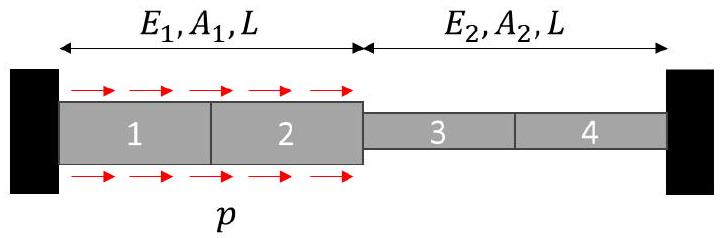
\includegraphics[max width=\textwidth, center]{2025_10_03_26e11264345fd9bad5cag-1(1)}
\end{center}
Maillage 1
\begin{center}
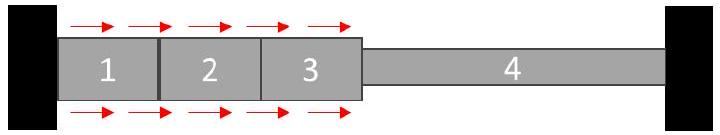
\includegraphics[max width=\textwidth, center]{2025_10_03_26e11264345fd9bad5cag-1}
\end{center}

Maillage 2
\begin{center}
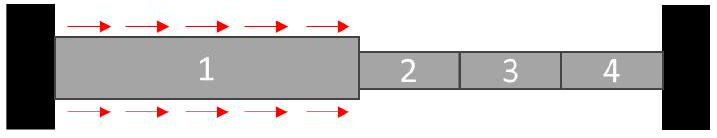
\includegraphics[max width=\textwidth, center]{2025_10_03_26e11264345fd9bad5cag-1(3)}
\end{center}

Maillage 3

\begin{enumerate}[start=7]
  \item Pour le maillage choisi, déterminer les matrices de rigidités élémentaires (applications numériques en kN/m)\\
  \item En déduire la matrice de raideur globale de la structure.\\
  \item Déterminer les forces nodales provoquées par le chargement.\\
  \item Etablir la relation $\{F\}=[K]\{d\}$ pour l'ensemble de la structure et résoudre les inconnues de déplacements.\\
  \item Tracer ainsi le champ de déplacements obtenu par la FEM et comparer au champ exact.\\
  \item En déduire le champ de contraintes obtenu par la FEM et comparer au champ exact. Quel enseignement peut-on en tirer ?
\end{enumerate}

\ifthenelse{\boolean{showSolutions}}{
\section*{ELEMENTS DE REPONSE}
\section*{1 Question 1}
En procédant à une coupure à gauche d'une section $\Sigma(\mathrm{x})$, il vient :

\begin{itemize}
  \item Pour $x<L$ :\\
$N(x)=X_{1}+p$\\
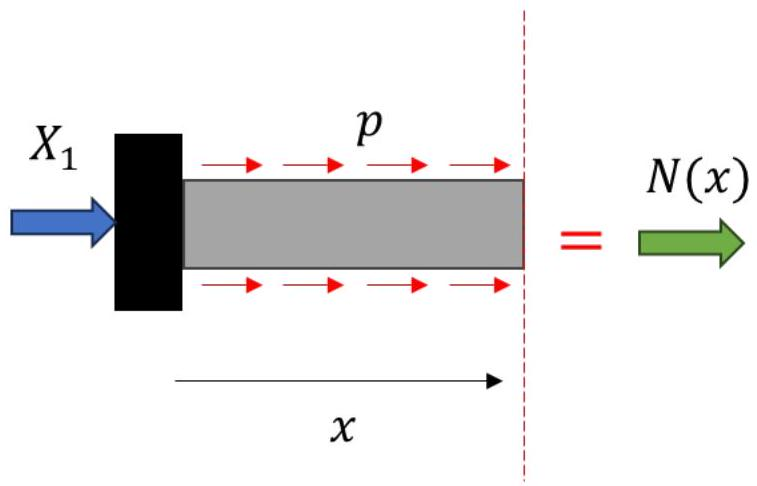
\includegraphics[max width=\textwidth, center]{2025_10_03_26e11264345fd9bad5cag-3}
  \item Pour $x>L$ :
\end{itemize}

$$
N(x)=X_{1}+p L
$$

\section*{2 Question 2}
D'après la loi de Hooke :

$$
\varepsilon(x)=\frac{d u(x)}{d x}=-\frac{\sigma(x)}{E(x)}=-\frac{N(x)}{E(x) A(x)}
$$

On en déduit alors la translation horizontale des sections à une abscisse x donnée :

\begin{itemize}
  \item Pour $x<L$ : on est dans la $1^{\text {ère }}$ barre en acier :
\end{itemize}

$$
u(x)=u_{A}-\int_{0}^{x} \frac{N(\xi)}{E_{1} A_{1}} d \xi=u_{A}-\int_{0}^{x} \frac{X_{1}+p \xi}{E_{1} A_{1}} d \xi=u_{A}-\frac{1}{E_{1} A_{1}}\left(X_{1} x+\frac{p x^{2}}{2}\right)
$$

On pourra noter que le déplacement en $\mathrm{x}=\mathrm{L}$ vaut alors :

$$
u(L)=u_{B}=u_{A}-\frac{1}{E_{1} A_{1}}\left(X_{1} L+\frac{p L^{2}}{2}\right)
$$

\begin{itemize}
  \item Pour $\mathrm{x}>\mathrm{L}$, on est dans la $2^{\text {nde }}$ barre en aluminium et l'effort normal est constant :
\end{itemize}

En se mettant dans le repère local de la seconde barre ( $\mathrm{x}=0$ au début de la $2^{\text {nde }}$ barre), il vient :

$$
u^{\prime}(x)=u_{B}-\int_{0}^{x} \frac{N(\xi)}{E_{2} A_{2}} d \xi=u_{B}-\int_{0}^{x} \frac{X_{1}+p L}{E_{2} A_{2}} d \xi=u_{A}-\frac{1}{E_{1} A_{1}}\left(X_{1} L+\frac{p L^{2}}{2}\right)-\frac{1}{E_{2} A_{2}}\left(X_{1} x+\frac{p L x}{2}\right)
$$

Le déplacement de l'extrémité de la seconde barre vaut alors :

$$
u^{\prime}(L)=u_{B}=u_{A}-\frac{1}{E_{1} A_{1}}\left(X_{1} L+\frac{p L^{2}}{2}\right)-\frac{1}{E_{2} A_{2}}\left(X_{1} L+\frac{p L^{2}}{2}\right)
$$

Or, d'après les conditions aux limites : $u_{A}=u_{B}=0$\\
On en déduit alors l'expression de la réaction $X_{1}$ :\\
Soit :

$$
X_{1} L\left(\frac{1}{E_{1} A_{1}}+\frac{1}{E_{2} A_{2}}\right)+p L^{2}\left(\frac{\frac{1}{2}}{E_{1} A_{1}}+\frac{1}{E_{2} A_{2}}\right)=0
$$

On note que $E_{1} A_{1}=E_{2} A_{2}=E A=210 M N$. On en déduit alors :

$$
\frac{2 X_{1}}{E A}+\frac{1.5 p L}{E A}=0
$$

Soit

$$
X_{1}=-\frac{3}{4} p L=0.75 * 100 * 6=-450 \mathrm{kN}
$$

On déduit également :

$$
X_{5}=p L-X_{1}=\frac{p L}{4}=150 \mathrm{kN}
$$

\section*{3 Question 3}
On en déduit l'allure de l'effort normal :

Pour $x<L: N(x)=-450+100 x$\\
Pour $x>L: N(x)=-450+600=150 k N$\\
Ci-dessous l'allure de l'effort normal :\\
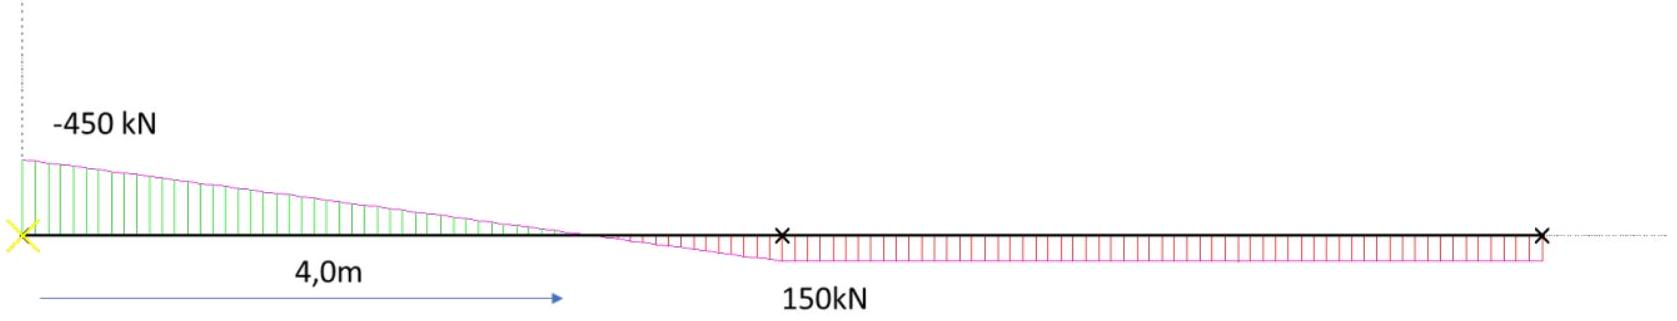
\includegraphics[max width=\textwidth, center]{2025_10_03_26e11264345fd9bad5cag-4}

On peut noter que la barre est en traction sur les 4 premiers mètres, puis en compression.

\section*{4 Question 4}
Le champ de déplacement se déduit des équations de Bresse :

$$
u(x)=u_{A}-\int_{0}^{x} \frac{N(\xi)}{E A} d \xi
$$

Où $u_{A}=0$ compte tenu de l'encastrement.\\
Ainsi, pour $x<L$ :

$$
u(x)=-\int_{0}^{x} \frac{-0.75 p L+p \xi}{E A} d \xi=\frac{p}{E A}\left(\frac{3 L x}{4}-\frac{x^{2}}{2}\right)
$$

En $x=L$, on note ainsi que :

$$
u(L)=\frac{1}{4} \frac{p L^{2}}{E A}
$$

Pour $x>L$ :

$$
u(x)=u(L)-\int_{L}^{x} \frac{0.25 p L}{E A} d \xi=\frac{1}{4} \frac{p L^{2}}{E A}-\frac{1}{4} \frac{p L}{E A}(x-L)
$$

On vérifie bien ainsi que

$$
u(2 L)=0
$$

Ci-dessous l'allure du champ de déformation. Il a une allure parabolique sur la première partie de la barre et une allure linéaire sur la seconde partie. On note que le déplacement maximal est obtenu en $x=3,75 m$, correspondant au point séparant le domaine des tractions et des compressions.

Pour cette abscisse $x=\frac{3}{4} L$, il vient :

$$
u_{\max }=\frac{9}{32} \frac{p L^{2}}{E A}=4,762 \times 10^{-3} m
$$

\begin{center}
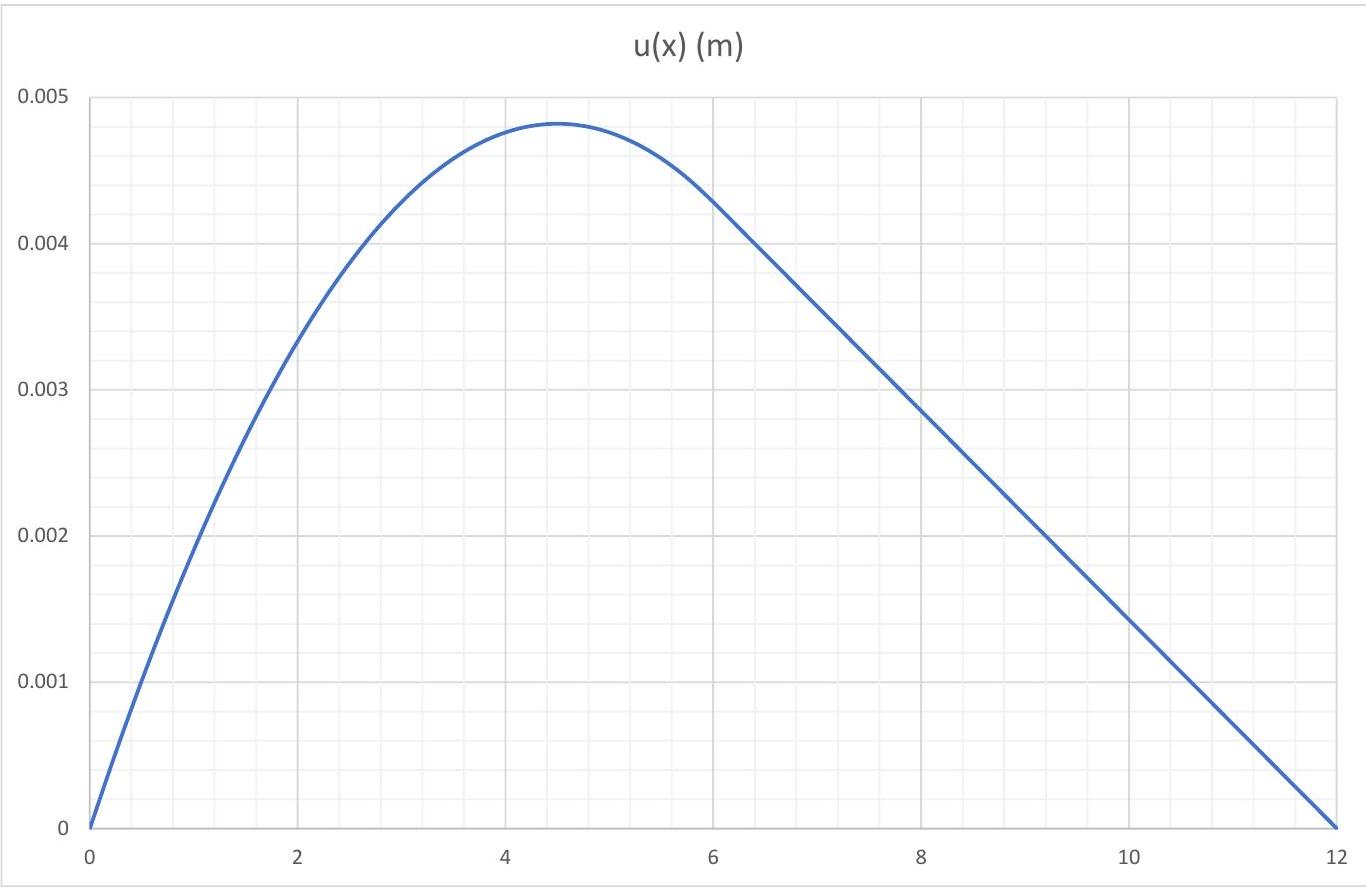
\includegraphics[max width=\textwidth]{2025_10_03_26e11264345fd9bad5cag-5}
\end{center}

\section*{5 Question 5}
Les contraintes dans la barre sont obtenues par la loi de Hooke:

$$
\sigma=-E \varepsilon=-E \frac{\partial u(x)}{\partial x}
$$

Ainsi, pour $x<L$ :

$$
\sigma=-\frac{p}{A_{1}}\left(\frac{3 L}{4}-x\right)
$$

La contrainte de traction est maximale à l'encastrement gauche, et suit une évolution linéaire. Elle est nulle en $x=4 \mathrm{~m}$. On enregistre ensuite une contrainte de compression croissante jusque $x=5 \mathrm{~m}$, pour atteindre 150 MPa en $x=6 \mathrm{~m}$.

Et pour $x>L$ :

$$
\sigma=\frac{1}{4} \frac{p L}{A_{2}}=50 \mathrm{MPa}
$$

La contrainte devient constante dans la seconde moitié de la barre et vaut 50 MPa . On note une chute brutale de la contrainte entre $x=6-\varepsilon$ où la contrainte vaut 150 MPa et $x=6+\varepsilon$ où la contrainte vaut 50 MPa . Cela s'explique par le changement de section qui est trois fois plus importante dans la seconde moitié ( 50 $\mathrm{MPa} \times 3=150 \mathrm{MPa}$ ). Les hypothèses simplificatrices ne rendent pas bien compte du phénomène complexe de diffusion des contraintes dans cette zone de transition brutale. Les résultats de la RDM établis ici sont valables lorsqu'on se situe suffisamment loin de la zone de discontinuité de section (principe de Saint Venant).

Rem : on aurait pu également établir ce résultat par la relation $\sigma=\frac{N}{A}$, mais ce n'est pas l'esprit de la méthode des éléments finis.\\
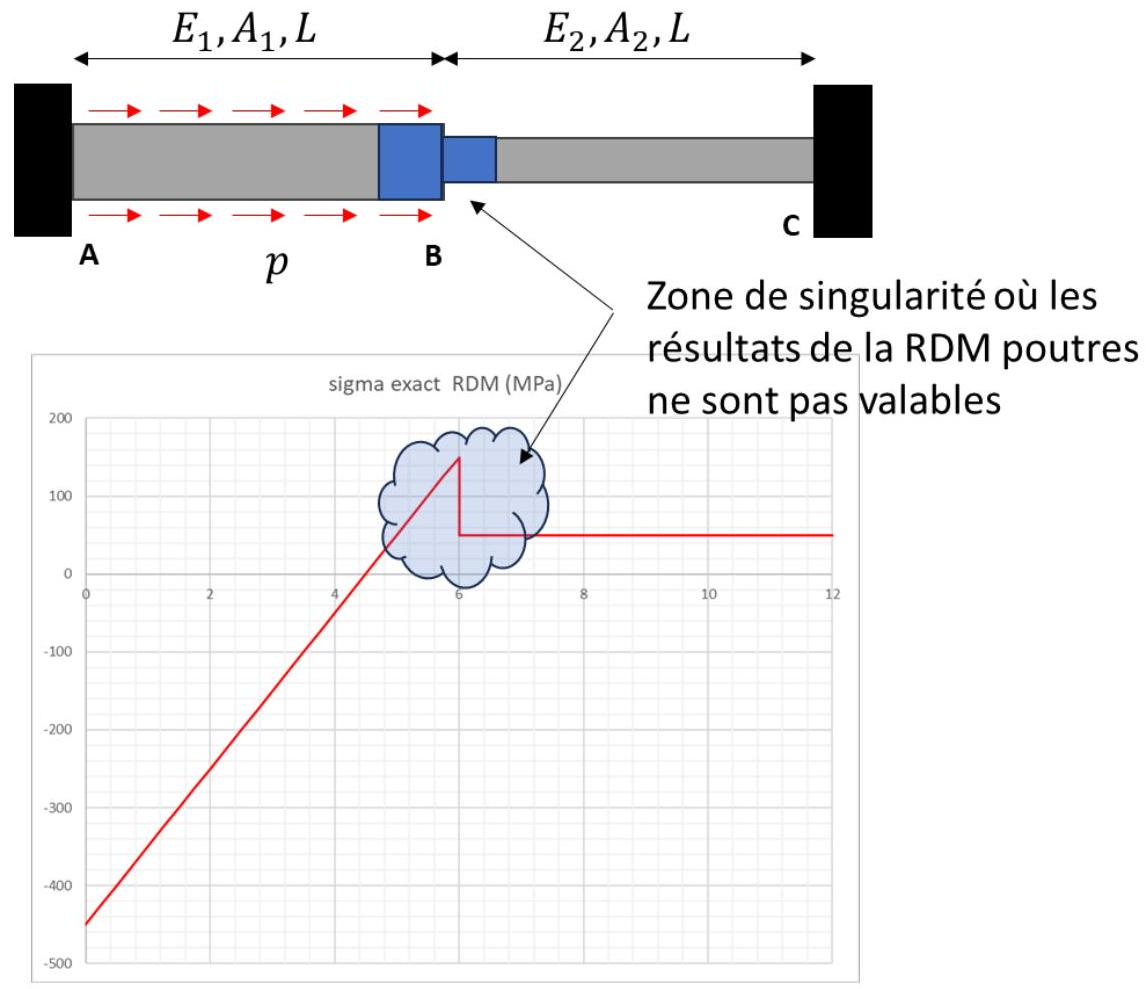
\includegraphics[max width=\textwidth, center]{2025_10_03_26e11264345fd9bad5cag-6}

\section*{6 Question 6}
Il n'y a pas de chargement dans la seconde moitié de la barre : cette seconde moitié ne sera soumis qu'à des efforts à ses extrémités, à savoir la réaction d'appui de droite ( $X_{5}$ ) et l'effort provenant de la partie au niveau de la jonction entre les 2 moitiés ( $X_{B}$ ). Les questions précédentes ont mis en évidence que la contrainte dans cette partie sont constantes. Il n'est donc pas nécessaire de discrétiser cette seconde moitié. En conséquence, le maillage 2 est le plus approprié car il permet une discrétisation de la première moitié de la poutre en 3 éléments et augmente donc ainsi la précision par rapport au maillage 1 ou au maillage 3.

\section*{7 Question 7}
On discrétise ainsi le $1^{\text {er }}$ tronçon en 3 éléments de 2 m et le second en un élément de 6 m .\\
Les matrices de rigidité élémentaire de chacun des tronçons 1,2 et 3 valent ainsi :

$$
K_{1}=K_{2}=K_{3}=\frac{E A_{1}}{L_{1} / 3}\left[\begin{array}{cc}
1 & -1 \\
-1 & 1
\end{array}\right]=\frac{3 E A_{1}}{L_{1}}\left[\begin{array}{cc}
1 & -1 \\
-1 & 1
\end{array}\right]=105000\left[\begin{array}{cc}
1 & -1 \\
-1 & 1
\end{array}\right](\mathrm{kN} / \mathrm{m})
$$

La matrice de rigidité élémentaire du tronçon 4 vaut ainsi :

$$
K_{4}=\frac{E A_{2}}{L_{2}}\left[\begin{array}{cc}
1 & -1 \\
-1 & 1
\end{array}\right]=35000\left[\begin{array}{cc}
1 & -1 \\
-1 & 1
\end{array}\right](\mathrm{kN} / \mathrm{m})
$$

\section*{8 Question 8}
La matrice de raideur est obtenue en procédant à l'assemblage des raideurs (voir cours sur les méthodes matricielles) :

$$
K=\left[\begin{array}{ccccc}
k_{1} & -k_{1} & 0 & 0 & 0 \\
-k_{1} & k_{1}+k_{2} & -k_{2} & 0 & 0 \\
0 & -k_{2} & k_{2}+k_{3} & -k_{3} & 0 \\
0 & 0 & -k_{3} & k_{3}+k_{4} & -k_{4} \\
0 & 0 & 0 & -k_{4} & k_{4}
\end{array}\right]=35000\left[\begin{array}{lrcrr}
3 & -3 & 0 & 0 & 0 \\
-3 & 6 & -3 & 0 & 0 \\
0 & -3 & 6 & -3 & 0 \\
0 & 0 & -3 & 4 & -1 \\
0 & 0 & 0 & -1 & 1
\end{array}\right]
$$

\section*{9 Question 9}
II a été montré en cours que le chargement nodal équivalent au chargement réparti p vaut $\frac{p L_{e}}{2}=100 \times \frac{2}{2}= 100 k N$ où $L_{e}=2 m$ est la longueur des éléments de la première moitié. Le chargement réel peut ainsi être remplacé par le chargement nodal équivalent :\\
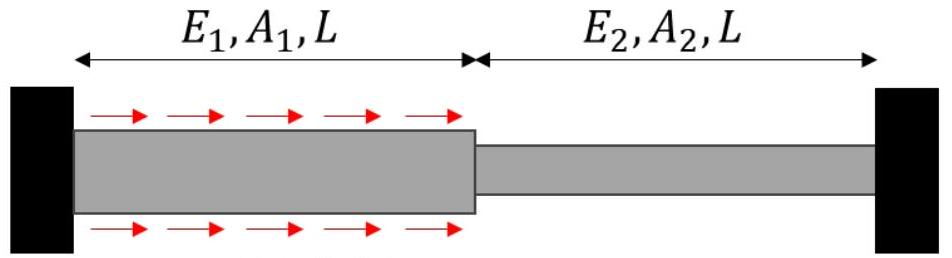
\includegraphics[max width=\textwidth, center]{2025_10_03_26e11264345fd9bad5cag-7(1)}

Chargement réel

$$
p=100 \mathrm{kN} / \mathrm{m}
$$

\begin{figure}[h]
\begin{center}
  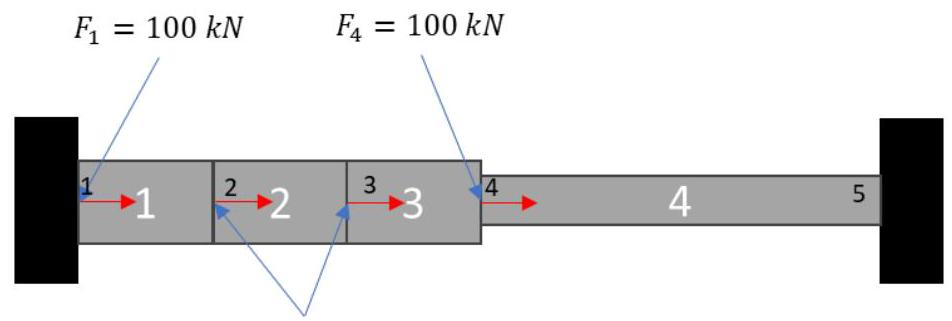
\includegraphics[width=\textwidth]{2025_10_03_26e11264345fd9bad5cag-7}
\captionsetup{labelformat=empty}
\caption{Maillage 2}
\end{center}
\end{figure}

$$
F_{2}=F_{3}=200 \mathrm{kN}
$$

On vérifie que la résultante du chargement réel est bien identique à celle des forces nodales équivalentes, soit 600 kN .

\section*{10 Question 10}
La relation force-déplacement de la structure est ainsi exprimé sous la force matricielle :

\begin{center}
\begin{tabular}{|l|l|l|l|l|l|l|l|l|}
\hline
\{F\} &  & u1 & 42 & u3 & u4 & u5 &  & \{d\} \\
\hline
X1 + 100 &  & $1.050 \mathrm{E}+05$ & $-1.050 \mathrm{E}+05$ & $0.000 \mathrm{E}+00$ & $0.000 \mathrm{E}+00$ & 0.000E+00 & \multirow{5}{*}{=} & u1 \\
\hline
200 &  & $-1.050 \mathrm{E}+05$ & $2.100 \mathrm{E}+05$ & $-1.050 \mathrm{E}+05$ & $0.000 \mathrm{E}+00$ & 0.000E+00 &  & u2 \\
\hline
200 & \multirow[t]{3}{*}{=} & 0.000E+00 & $-1.050 \mathrm{E}+05$ & $2.100 \mathrm{E}+05$ & $-1.050 \mathrm{E}+05$ & 0.000E+00 &  & u3 \\
\hline
100 &  & 0.000E+00 & $0.000 \mathrm{E}+00$ & $-1.050 \mathrm{E}+05$ & $1.400 \mathrm{E}+05$ & -3.500E+04 &  & u4 \\
\hline
X5 &  & $0.000 \mathrm{E}+00$ & $0.000 \mathrm{E}+00$ & $0.000 \mathrm{E}+00$ & $-3.500 \mathrm{E}+04$ & $3.500 \mathrm{E}+04$ &  & u5 \\
\hline
\end{tabular}
\end{center}

Où les forces inconnues sont les réactions d'appui $X_{1}$ et $X_{5}$. Au niveau des appuis, en revanche on sait que $u_{1}=u_{5}=0$.

Les inconnues de déplacement sont résolues en inversant la relation $\{F\}=[K]\{d\}$ où les lignes et colonnes correspondant au dd connus sont supprimées (en grisé) :

\begin{center}
\begin{tabular}{|l|l|l|l|l|l|l|l|l|l|}
\hline
\{F\} &  & u1 & 42 & 43 & u4 & 45 &  & \{d\} & \{ drésolu\} \\
\hline
X1 + 100 &  & $1.050 \mathrm{E}+05$ & -1.050E+05 & $0.000 \mathrm{E}+00$ & $0.000 \mathrm{E}+00$ & $0.000 \mathrm{E}+00$ & \multirow{5}{*}{=} & u1 & 0.00E+00 \\
\hline
200 &  & $-1.050 \mathrm{E}+05$ & $2.100 \mathrm{E}+05$ & -1.050E+05 & $0.000 \mathrm{E}+00$ & $0.000 \mathrm{E}+00$ &  & u2 & 3.33E-03 \\
\hline
200 & \multirow[t]{3}{*}{=} & $0.000 \mathrm{E}+00$ & $-1.050 \mathrm{E}+05$ & $2.100 \mathrm{E}+05$ & $-1.050 \mathrm{E}+05$ & 0.000E+00 &  & u3 & 4.76E-03 \\
\hline
100 &  & $0.000 \mathrm{E}+00$ & $0.000 \mathrm{E}+00$ & $-1.050 \mathrm{E}+05$ & $1.400 \mathrm{E}+05$ & $-3.500 \mathrm{E}+04$ &  & u4 & 4.29E-03 \\
\hline
X5 &  & $0.000 \mathrm{E}+00$ & $0.000 \mathrm{E}+00$ & $0.000 \mathrm{E}+00$ & $-3.500 \mathrm{E}+04$ & $3.500 \mathrm{E}+04$ &  & u5 & 0.00E+00 \\
\hline
\end{tabular}
\end{center}

\section*{11 Question 11}
Le champ de déplacement est donné ci-dessous et superposé au champ de déplacement exact.

On peut constater que le champ FEM est identique au champ exact dans la partie de barre non chargée. ll y a bien sûr un léger écart dans la partie de barre chargée. On pourra néanmoins noter que les déplacements FEM et exacts sont identiques aux niveaux des nœuds du maillage, à savoir en $x=0,2,4,6$ et 12 m .\\
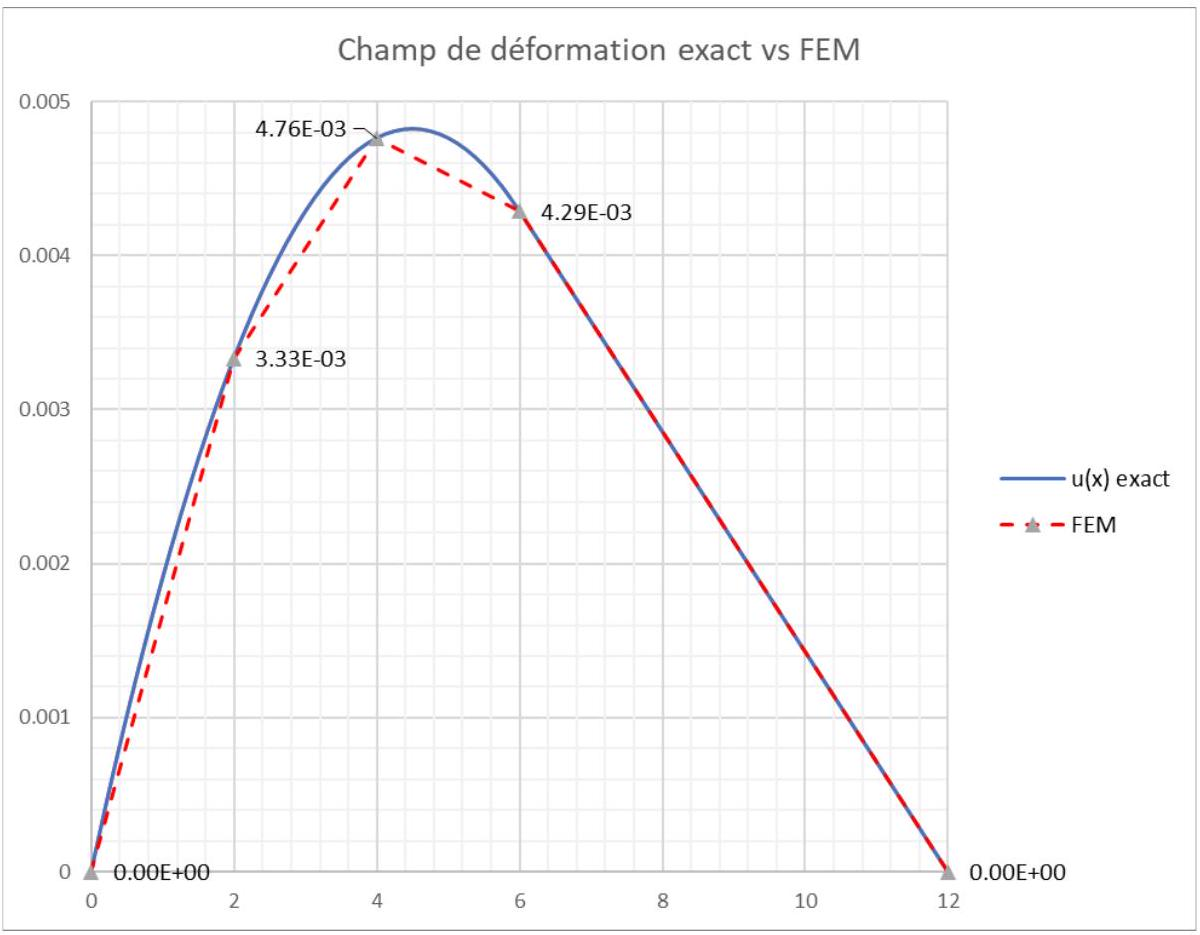
\includegraphics[max width=\textwidth, center]{2025_10_03_26e11264345fd9bad5cag-8}

\section*{12 Question 12}
Pour déterminer le champ de contrainte FEM, il convient d'établir d'abord les déformations dans chaque élément fini (origine i, extrémité j, longueur Lij) donné par la relation :

$$
\varepsilon=\frac{u_{j}-u_{i}}{L_{i j}}
$$

Puis d'appliquer la loi de Hooke (ici version GC, comme vue en cours de RDM) :

$$
\sigma=-E_{i j} \varepsilon=-E_{i j} \frac{u_{j}-u_{i}}{L_{i j}}
$$

Le tableau ci-dessous résume les valeurs nodales des contraintes :

\begin{center}
\begin{tabular}{|l|l|l|l|l|l|}
\hline
x & u(x) FEM & Le (m) & epsilon & E (MPa) & sigma FEM (MPa) \\
\hline
0 & 0 &  & 0.00166667 & 210000 & -350 \\
\hline
2 & 3.33E-03 & 2 & 0.00166667 & 210000 & -350 \\
\hline
4 & 4.76E-03 & 2 & 0.00071429 & 210000 & -150 \\
\hline
6 & 4.29 E -03 & 2 & -0.0002381 & 210000 & 50 \\
\hline
6 & 4.29 E -03 & 6 & -0.0007143 & 70000 & 50 \\
\hline
12 & 0.00E+00 & 6 & -0.0007143 & 70000 & 50 \\
\hline
\end{tabular}
\end{center}

Le graphique ci-dessous superpose les champs de contraintes exact et FEM :\\
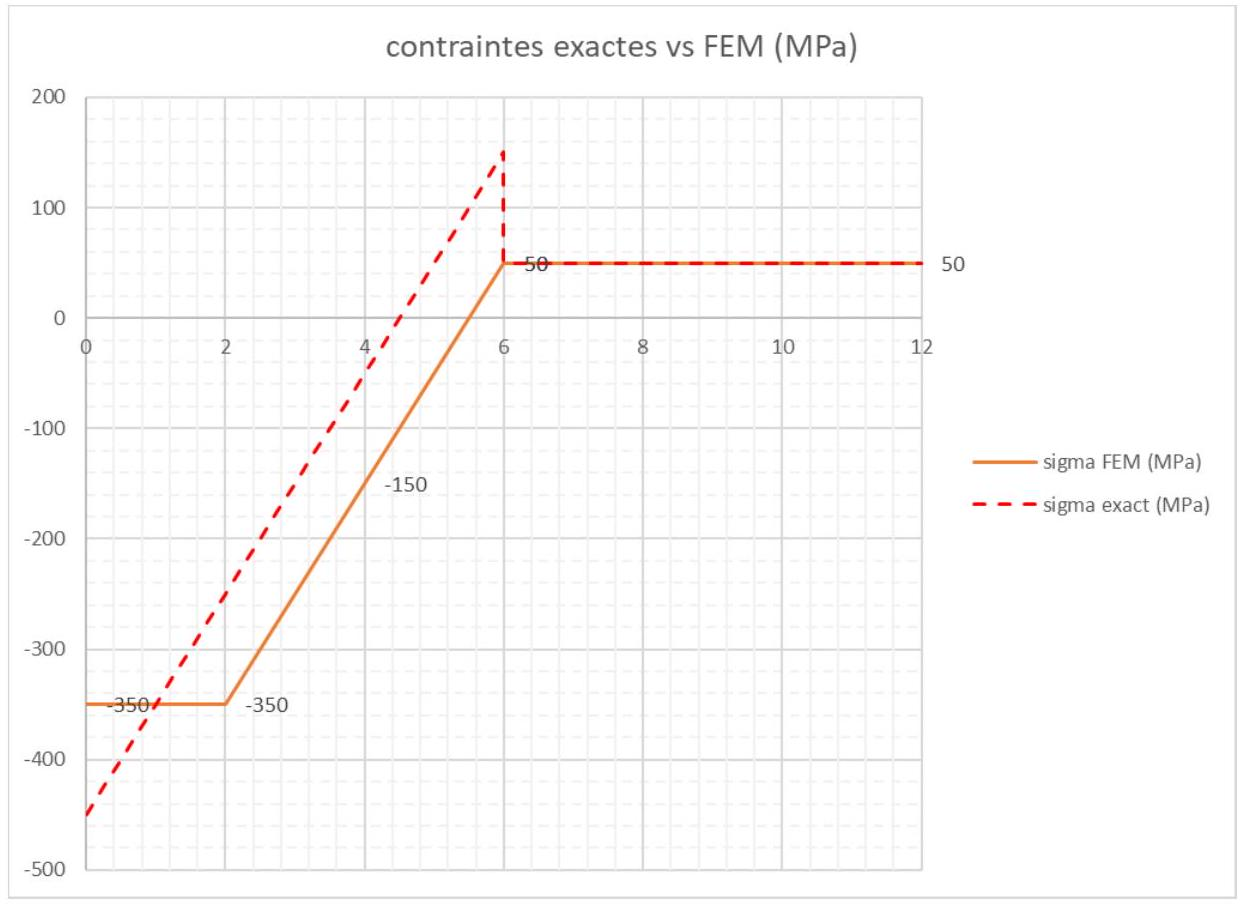
\includegraphics[max width=\textwidth, center]{2025_10_03_26e11264345fd9bad5cag-9}

Dans la seconde moitié de la barre, on retrouve exactement la même contrainte que la contrainte exacte, ce qui était attendu. En revanche, dans la première moitié, on trouve des différences très significatives. Cela s'explique par le fait que les contraintes sont proportionnelles aux déformations, donc proportionnelles aux dérivées du déplacement. Or on peut constater que si, qualitativement, on avait une bonne approximation du champ de déplacement, on s'aperçoit qu'il n'en est pas de même pour les dérivées (c'est-à-dire les pentes des courbes de champs de déplacement exact et FEM) : le graphique comparant les champs de déplacement montre en effet des pentes bien différentes, ce qui explique que les résultats sont beaucoup moins probants pour les déformations et les contraintes. Aussi, pour avoir des résultats meilleurs, il faut discrétiser encore plus la structure dans la zone chargée, les pentes du champ de déplacement donné par la FEM se rapprocheront des pentes du champ de déplacement exact. Cet exemple montre ainsi que lorsqu'on procède à une opération de dérivation à partir d'un champ approché, plus l'écart entre la dérivée du champ approché et la dérivée du champ exact (ici les champs de déformations ou contraintes) augmente, plus les écarts sur les contraintes, qui sont une des grandeurs qui guident en général la conception des ouvrages, augmentent.

Cet exemple montre aussi qu'un maillage « grossier » peut aboutir à une sous-estimation des contraintes.
}

\end{document}